\documentclass{beamer}

% balíčky

\usepackage[size=custom, width=120, height=120, scale=0.9, margin=0pt]{beamerposter}
\usepackage{socstyle}
\usepackage[absolute,overlay]{textpos}

\usepackage[font={footnotesize}]{caption}
\usepackage[font={footnotesize}]{subcaption}

\usepackage{multicol}

\usepackage{parskip}
\renewcommand{\baselinestretch}{1.1}
\setlength{\parskip}{18pt} 
% \renewcommand{\arraystretch}{0.5}

\usepackage{tcolorbox}
\tcbuselibrary{breakable}
\definecolor{myblue}{HTML}{172983}
\tcbset{
		colback=myblue!5!white,
		colframe=myblue!75!black,
		fonttitle=\fontsize{48}{35}\selectfont\bfseries,
		boxrule=5pt,
		boxsep=18pt,
		parbox=false
}

\usepackage{asymptote}
\def\asydir{asy}

\usepackage[backend=biber, url=true, style=numeric, sorting=none]{biblatex}
\usepackage{url}
\addbibresource{soc.bib}
\renewcommand*{\bibfont}{\footnotesize}

% délky
\newlength{\head}
\setlength{\head}{20cm}

\newlength{\sep}
\setlength{\sep}{1.5cm}

\newlength{\vyska}
\setlength{\vyska}{\paperheight}
\addtolength{\vyska}{-\head}

\newlength{\vyskaA}
\setlength{\vyskaA}{\vyska}
\addtolength{\vyskaA}{-2\sep}

\newlength{\vyskaB}
\setlength{\vyskaB}{\vyska}
\addtolength{\vyskaB}{-2\sep}

\newlength{\vyskaC}
\setlength{\vyskaC}{\vyska}
\addtolength{\vyskaC}{-2\sep}

\newlength{\side}
\setlength{\side}{30cm}
\addtolength{\side}{-2\sep}

\newlength{\main}
\setlength{\main}{60cm}
\addtolength{\main}{-2\sep}

\newlength{\newparskip}
\setlength{\newparskip}{12pt}

\setlength{\baselineskip}{82pt}

% témata
\usetheme{Rochester}
\usecolortheme{seahorse}

% posraný zarovnávání
\newlength{\headP}
\setlength{\headP}{\head}
\addtolength{\headP}{-\sep}
\setbeamertemplate{headline}{%
\leavevmode%
  \hbox{%
    \begin{beamercolorbox}[wd=\paperwidth,ht=\headP,dp=0pt]{bg=green}%
    \end{beamercolorbox}%
  }
}
\setbeamertemplate{footline}[frame number]{}
\setbeamertemplate{navigation symbols}{}
\setbeamertemplate{footline}{} 
\setbeamertemplate{bibliography item}{\insertbiblabel}

% asi naprd definice
\title{Mechanika rodin planetek \\ s aplikací na rodinu Eunomia}
\author{Adam Křivka \\ \and doc. Mgr. Miroslav Brož, Ph.\,D.}
\institute{Cyrilometodějské gymnázium a střední odborná škola pedagogická Brno,\\ Lerchova 63, 602 00 Brno}


% ----------


\begin{document}

\begin{frame}

\begin{columns}[t]

\begin{column}{\sep}
\end{column}
\begin{column}{\side}
	\begin{tcolorbox}[title=Asteroids in the Solar System\vphantom{Úy},height=0.335\vyskaA,parbox=false]
		\textbf{Asteroids} is the most numerous and also most interesting group of bodies in~\textbf{the Solar System}. The first asteroid was discovered in 1801 and more than half a million asteroids are known today.\\[\newparskip]

		In~\textbf{the main asteroid belt} between \textit{Mars} and~\textit{Jupiter}, asteroids form \textbf{families} --- groupings created by a initial \textbf{breakup} of the same parent body, caused by a collision with another body. In~our work, we focus on a large family called \textit{Eunomia}, located in the middle main belt.\\[\newparskip]

		By studying collisional families, we can find out more about the creation of the Solar System and its \textbf{dynamical structure}~\cite{nesvorny15}, for example we can support the \textbf{Late Heavy Bombardment} theory)~\cite{broz13}. \\[\newparskip]

		\vspace{3cm}

		\begin{figure}[!htb]
			\begin{subfigure}[t]{0.44\textwidth}
			\centering
			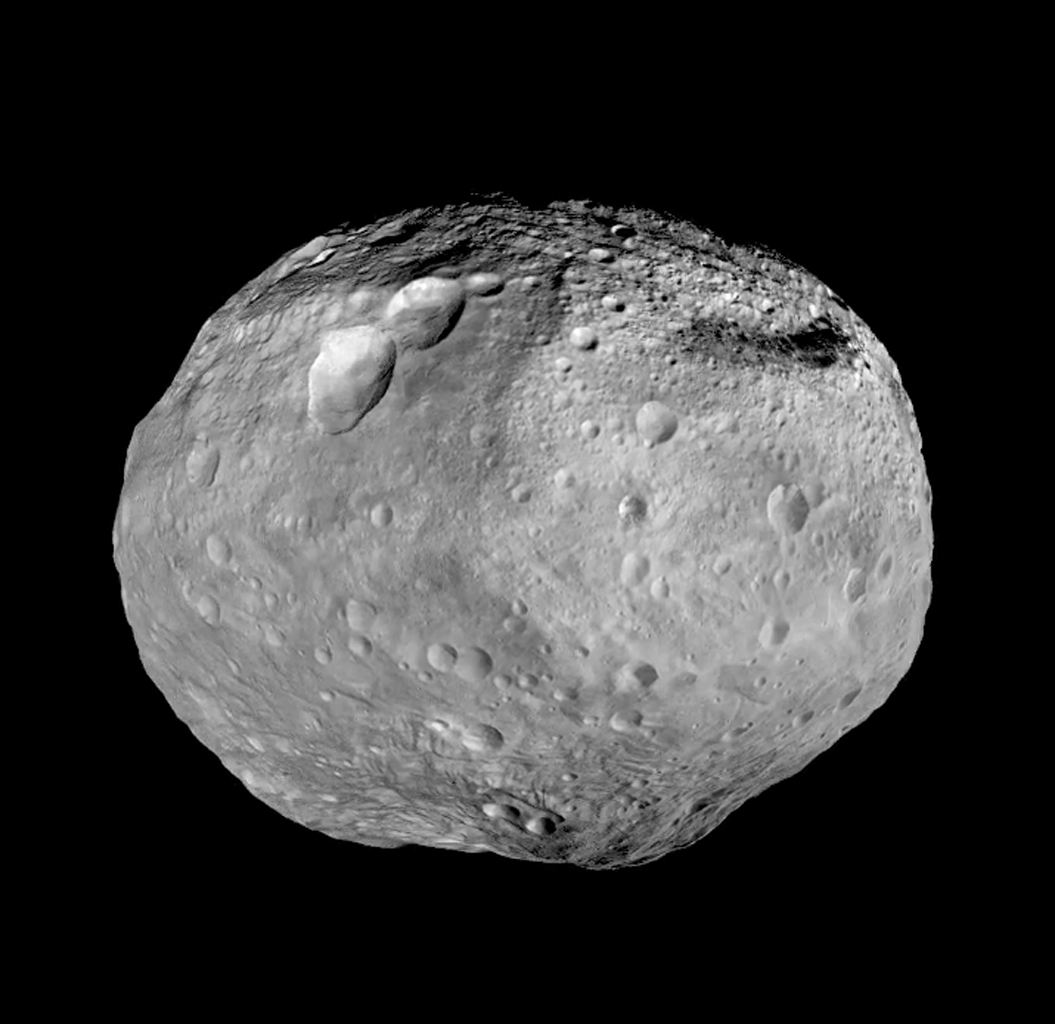
\includegraphics[width=0.95\textwidth]{../obr/vesta.jpg}
			\caption{Asteroid \textit{(4) Vesta} --- second largest and~ most massive body of the main belt.} \label{fig:vesta}
			\end{subfigure}
			\begin{subfigure}[t]{0.55\textwidth}
			\centering
			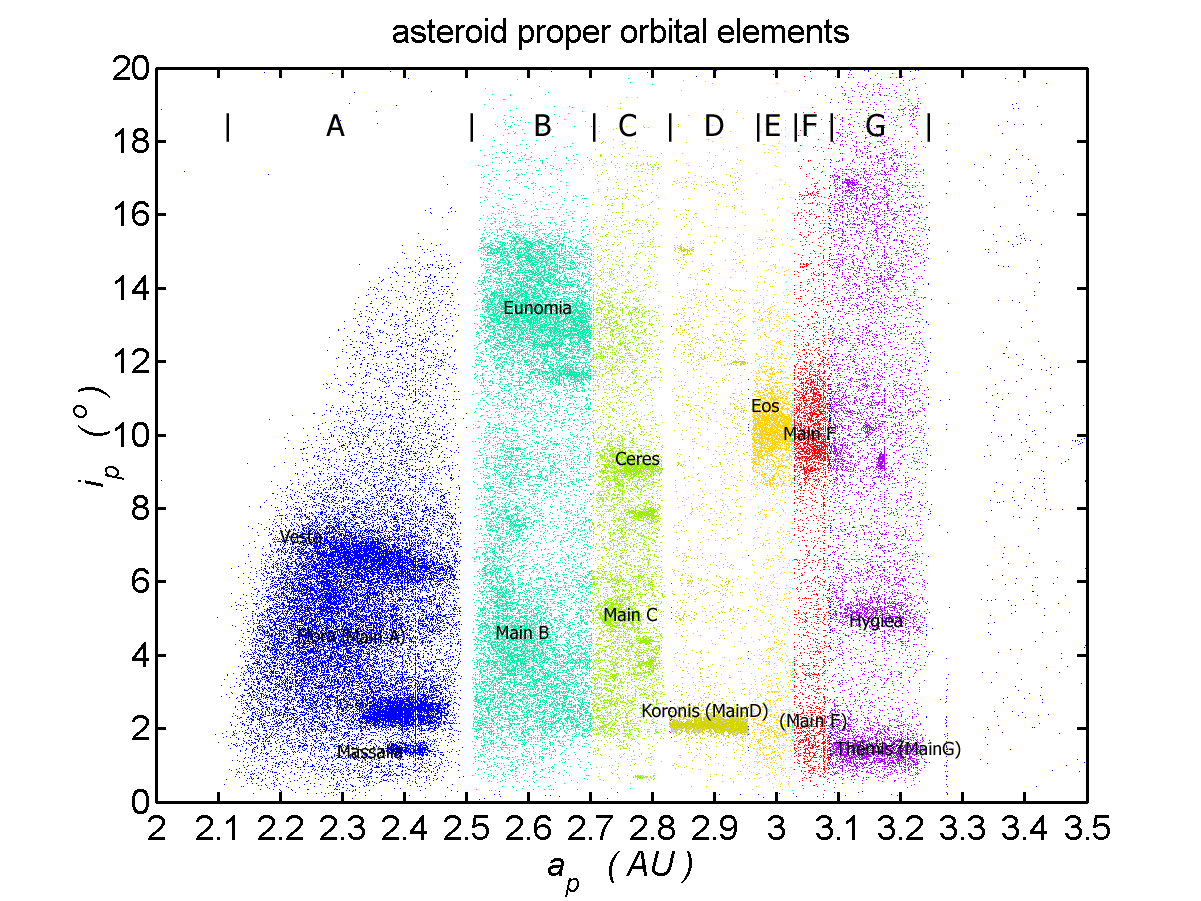
\includegraphics[width=1.0\textwidth]{../obr/mainbelt.png}
			\caption{Main asteroid belt in the space of \textbf{proper orbital elements} --- proper semi-major axis $a_{\rm p}$ and proper inclination. $\sin I_{\rm p}$.} \label{fig:belt}
			\end{subfigure}
		\end{figure}
	\end{tcolorbox}

\vspace{\sep}

	\begin{tcolorbox}[title=Methods of celestial mechanics\vphantom{Úy},height=0.665\vyskaA]

		The fundamental problem of celestial mechanics is the \textbf{N-body problem} --- calculate the position of bodies, that are gravitationally bound together according Newton's law of universal gravitation, at any time.

		{\footnotesize
		\begin{align*} 
			\vec{F}_i = m_i\vec{a}_i &= -\sum_{\substack{j=1 \\ j\neq i}}^N G\frac{m_im_j}{\abs{\vec{r}_i-\vec{r}_j}^3}(\vec{r_i}-\vec{r_j})\,, \qquad{\rm pro}\ i\in\{1,\,2,\,\dots,\,N\}
		\end{align*}}

		For simulation of orbital evolution, we use a \textbf{\it numerical integrator SWIFT}, which counts with  

	% \itemsep0em
\begin{itemize}
	\item \textbf{Yarkovsky effect},
	\item \textbf{YORP effect},
	\item \textbf{random collisions},
	\item \textbf{chaotic diffusion}.  
\end{itemize}

		\begin{figure}[!htb]
			\centering 
			\begin{subfigure}[b]{0.45\textwidth}
			\centering 
			\asyinclude[width=1.0\textwidth]{../asy/f_euler.asy}
			\end{subfigure}
			\begin{subfigure}[b]{0.45\textwidth}
			\centering 
			\asyinclude[width=1.0\textwidth]{../asy/b_euler.asy}
			\end{subfigure}
			\caption{Illustration of a simpler integration method --- \textbf{Euler's method} --- which is in principle similar to ours.}
		\end{figure}
		% \vspace{36pt}
		The orbit around the Sun of an asteroid can be described with \textbf{orbital elements}:
		\vspace{-12pt}
		\begin{itemize}
			% \itemsep0em
			\item \textbf{semi-major axis} $a$
			\item \textbf{eccentricity} $e$
			\item \textbf{inclination} $I$ (or also $\sin I$) 
		\end{itemize}
		\vspace{-12pt}

\vspace{1cm}

They are subject to change by \textbf{perturbations} (e.g. gravitational forces of other planets); we can thus \enquote{average} them over long periods to \textbf{mean} and to \textbf{proper orbital elements}, where the latter are not subject to any periodical forces.

		\vspace{1.0cm}

		\begin{figure}
			\centering
			\begin{subfigure}[b]{0.49\textwidth}
			\centering
			\includegraphics[width=1.0\textwidth]{../obr/atOF_en}
			\end{subfigure}
			\begin{subfigure}[b]{0.49\textwidth}
			\centering
			\includegraphics[width=1.0\textwidth]{../obr/atFP_en}
			\end{subfigure}
			\caption{\ Comparison of \textbf{osculating} (actual) and \textbf{mean} semi-major axis (left), and \textbf{mean} and \textbf{proper} semi-major axis (right) for one particle simulated for $3.76$ million years.}
		\end{figure}
		% \vspace{-48pt}
		\begin{tabularx}{\textwidth}{p{12cm}X}

		\

		For identification of members of a family, we use the \textbf{hierarchical clustering method} (HCM): in the phase space  $(a_{\rm p},\,e_{\rm p},\sin I_{\rm p})$ we choose a cut-off \enquote{distance} of bodies $v_{\rm cutoff}$ (with units of velocity), according to which, beginning with the parent body \textit{(15) Eunomia}, we then determine the members.
		&
		\begin{figure}
			\centering
			\includegraphics[width=0.4\textwidth]{../obr/Nv_edit_en.png}
			\caption{Dependence of the number of the members of the family \textit{Eunomia} on the chosen cut-off velocity $v_{\rm cutoff}$ while using the HCM.}
		\end{figure}
		\end{tabularx}
		\vspace{-0.5cm}
		{\begin{align*}
			v_{\rm cuttoff}=na_{\rm p}\sqrt{C_a\left(\frac{\Delta a_{\rm p}}{a_{\rm p}}\right)^2+C_e(\Delta e_{\rm p})^2+C_i(\Delta \sin i_{\rm p})^2}
		\end{align*}}

	\end{tcolorbox}

\vspace{\sep}

\end{column}

\begin{column}{2\sep}
\end{column}

\begin{column}{\main}
\begin{tcolorbox}[title=Identification of members of the Eunomia family\vphantom{Úy},height=0.25\vyskaB]

	For determining the \textit{Eunomia} family, we used the clustering algorithm. Then, we removed \textbf{interlopers} using the relationship between \textbf{semi-major axis drift} $\Delta a_{\rm p}$ and \textbf{absolute magnitude} $H$, and using two spectroscopic methods --- the relationship of \textbf{albedoes} $p_{\rm V}$ a $p_{\rm IR}$ and the relationship of \textbf{color indexes} $a^*$ a $i-z$. Before the removal, the member count was 6503; after using all the mentioned methods it was 6184.

	\vspace{-1.7cm}

	\begin{figure}[htbp]
		\begin{subfigure}[b]{0.3\textwidth}
			\centering
			\captionsetup{width=.88\linewidth}
			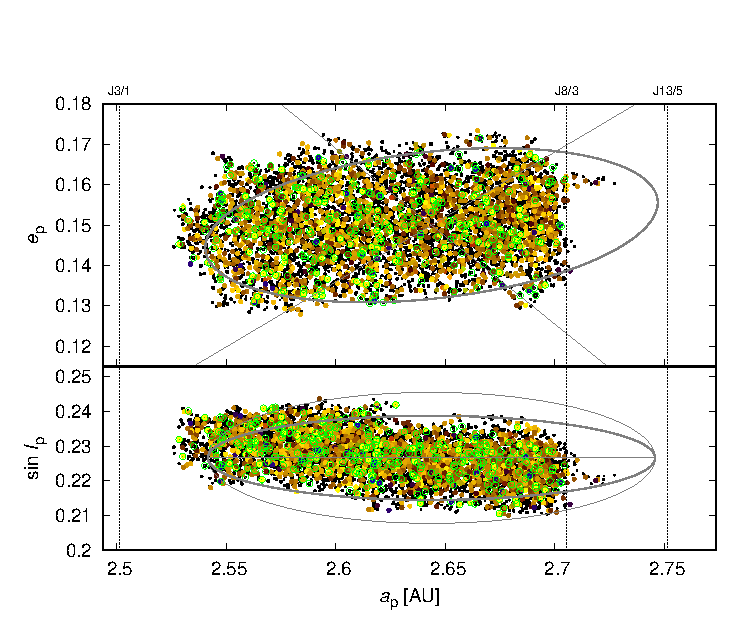
\includegraphics[width=1.0\textwidth]{../obr/ae_ai_wise}
			\caption{Observed \textit{Eunomia} family identified by HCM with $v_{\rm cutoff} = 44\,{\rm m/s}$ in~space of \textbf{proper semi-major axis} $a_{\rm p}$ and~\textbf{proper eccentricity} $e_{\rm p}$ (top) and~in~space of \textbf{proper semi-major axis} $a_{\rm p}$ and~\textbf{proper inclination} $\sin I_{\rm p}$ (bottom). The color code is adapted from the \textbf{albedoes} $p_{\rm V}$ and~$p_{\rm IR}$ from the WISE  catalogue\cite{nugent15}.}
			\label{fig:ae_ai_wise}
		\end{subfigure}
		\begin{subfigure}[b]{0.26\textwidth}
			\centering
			\captionsetup{width=.88\linewidth}
			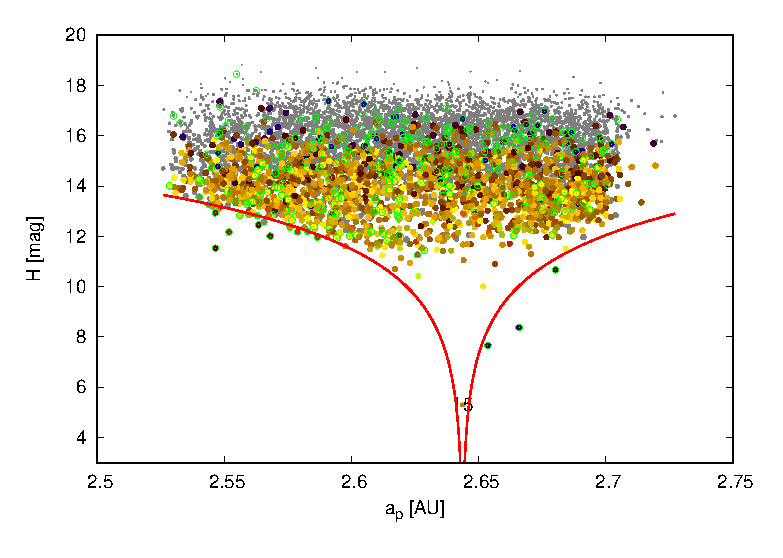
\includegraphics[width=1.0\textwidth]{../obr/aH_wise}
			\caption{\textbf{Proper semi-major axis} $a_{\rm p}$ versus~\textbf{absolute magnitude} $H$. We can see a typical \enquote{V}-shape, which is caused by an initial \textbf{velocity field} and the~\textbf{Yarkovsky effect}, which is even magnified by the \textbf{YORP effect}, which leads to an increased concentration of small asteroids at the edges of the family.\newline\newline}

		\end{subfigure}
		\begin{subfigure}[b]{0.2\textwidth}
			\centering
			\captionsetup{width=.88\linewidth}
			\includegraphics[width=1.0\textwidth]{../obr/pV_pIR-crop}
			\caption{\textbf{Albedoes} $p_{\rm V}$ (in the visible spectrum) and~$p_{\rm IR}$ (in infrared) from the WISE catalogue. The colors don't resemble real color. For identification of \textbf{interlopers}, the following values were chosen $0,05 \leq p_{\rm V} \leq 0,4$.\newline}
		\end{subfigure}
		\begin{subfigure}[b]{0.2\textwidth}
			\centering
			\captionsetup{width=.88\linewidth}
			\includegraphics[width=1.0\textwidth]{../obr/astar_iz-crop}
			\caption{\textbf{Color indexes} $a^*$ and~$i-z$ from the Sloan catalogue\cite{ivezic01}. The colors don't resemble real color. For identification of \textbf{interlopers}, the following values were chosen $0\leq a^* \leq 0,3$ a~$-0,3\leq i-z \leq 0,3$.\newline\newline}
		\end{subfigure}
	\end{figure}

\end{tcolorbox}

\vspace{\sep}

\begin{tcolorbox}[title=Simulation of orbital evolution\vphantom{Úy},height=0.75\vyskaB]
	\begin{tabularx}{\textwidth}{Xp{0.25\textwidth}}

	When creating the \textbf{synthetic} population of asteroids, we assigned the following properties to the particles
	\begin{itemize}
	% \itemsep0em
	\item \textbf{diameters} (from observed data --- we took the \textbf{size-frequency distribution} into account), 
	\item \textbf{albedoes} (from observed data),
	\item \textbf{rotational axis orientations} (randomly; influence on the \textbf{Yarkovsky effect}),
	\item \textbf{initial velocities} (simulating an \textbf{isotropic breakup} at the location on the orbit with values $f=90^\circ$ and $\omega+f=50^\circ$).
	\end{itemize}

\

	We simulated a population of \textbf{6210 particles} for \textbf{$1,3$ billion years}. The computation was run on a \textbf{server of the Astronomical Institute of Charles University}; it took around  \textbf{50000 CPU hours} and and the total amount of \textbf{binary data} was $3\,{\rm GB}$.


		&

		\vspace{-1cm}
		\begin{figure}
			\centering
			\captionsetup{width=0.2\textwidth}
			\includegraphics[width=0.2\textwidth]{../obr/size_distribution_en}
			\caption{\textbf{Size-frequency distribution} of the \textit{Eunomian} asteroids.} 

			\label{fig:sfd}
		\end{figure}
	\end{tabularx}

	\begin{figure}[t]
		\centering
		\includegraphics[width=0.24\textwidth]{../obr/pngB_en/ae_5.png}
		\includegraphics[width=0.24\textwidth]{../obr/pngB_en/ae_205.png}
		\includegraphics[width=0.24\textwidth]{../obr/pngB_en/ae_605.png}
		\includegraphics[width=0.24\textwidth]{../obr/pngB_en/ae_1105.png}
\\
		\includegraphics[width=0.24\textwidth]{../obr/pngB_en/ai_5.png}
		\includegraphics[width=0.24\textwidth]{../obr/pngB_en/ai_205.png}
		\includegraphics[width=0.24\textwidth]{../obr/pngB_en/ai_605.png}
		\includegraphics[width=0.24\textwidth]{../obr/pngB_en/ai_1105.png}
\\
		\includegraphics[width=0.24\textwidth]{../obr/pngB_en/ei_5.png}
		\includegraphics[width=0.24\textwidth]{../obr/pngB_en/ei_205.png}
		\includegraphics[width=0.24\textwidth]{../obr/pngB_en/ei_605.png}
		\includegraphics[width=0.24\textwidth]{../obr/pngB_en/ei_1105.png}
			\captionsetup{width=.88\linewidth}
			\caption{Results of the simulation in~space of $(a_{\rm p},\,e_{\rm p})$, $(a_{\rm p},\,\sin I_{\rm p})$ and  $(e_{\rm p},\,\sin I_{\rm p})$ at~times $t=5,\,205,\,605,\,1105$ million year. The labels J3/1, J8/3, J13/5 a~J5/2 indicate the most significant \textbf{resonances} with~\textit{Jupiter}. The black line at the top indicates the edge of the region, where the asteroid's orbit crosses \textit{Mars'}. A similar border exists for \textbf{Jupiter} as well, but it is located outside these graphs (at $e=0,65$). The purple rectangle labels the region chosen for a sample for the \textbf{background} population.} \label{fig:ae_sim}
	\end{figure}

\begin{multicols}{2}

\begin{itemize}
\item 
Due to the specific \textbf{proper elements} calculation process from initial velocities, at $t=5$ million years, we can see a slightly unsymmetrical shape of the simulated family. 

\item The mechanism, through which the asteroids \textbf{leave} the family is the following: due to the \textbf{Yarkovsky effect}, the asteroid gets close to a \textbf{resonance}, the eccentricity of its orbit \textbf{increases} until it starts to \textbf{cross the orbit} of \textit{Mars} or \textit{Jupiter}, whereat due to a \textbf{close encounter} it gets swung out of its orbit.

\vspace{1cm}
	\begin{figure}
		\centering
		\includegraphics[width=0.25\textwidth]{../obr/ae_obs.png}
		\caption{Graph $(a_{\rm p}, e_{\rm p})$ for the observed \textit{Eunomia} family. The color code indicates the number of particles in the given \textbf{box}.}
	\end{figure}
\vfill\null\columnbreak

\item The asteroids initially located near the J5/2 resonance, were very quickly diffused, thus they are not present at the $t=5\,{\rm My}$ graph.

\item \textbf{Resonances} J8/3 and~J13/5 clearly divide the family into three parts, which have different widths, and thus the asteroids in them get diffused at different rates.

\item It is confirmed, that the J8/3 \textbf{resonance} is stronger than the J13/5 \textbf{resonance} (asteroids near the J8/3 resonance at $t=205\,{\rm My}$  got diffused into a region of width $0,05<e_{\rm p}<0,5$, while near the J13/5 resonance, they reached only $0,1<e_{\rm p}<0,23$)

\item At the $(a_{\rm p},\,\sin I_{\rm p})$ graph, we can observe a slight \enquote{\textbf{tilt}} of the observer family (the part under $a\approx2,62\,{\rm AU}$ has a higher inclination $I_{\rm p}$), which we can unfortunately not yet spot on the simulated family.

\item With time, the concentration of asteroids in space \textbf{decreases}, which is caused by \textbf{all} the present \textbf{resonances}.

\end{itemize}
\end{multicols}

\vspace{-1cm}

	\begin{figure}
		\centering
		\includegraphics[width=0.24\textwidth]{../obr/ae_scl_0006.png}
		\includegraphics[width=0.24\textwidth]{../obr/ae_scl_0206.png}
		\includegraphics[width=0.24\textwidth]{../obr/ae_scl_0606.png}
		\includegraphics[width=0.24\textwidth]{../obr/ae_scl_1106.png}
		\captionsetup{width=.88\linewidth}
		\caption{$(a_{\rm p},\,e_{\rm p})$ graph of the simulated \textit{Eunomia} family for $t=5,\ 205,\ 605, 1105$ million years. Notice the change in the color code.} 

		\label{fig:ae_chi2}
	\end{figure}

\vspace{1.5cm}

\end{tcolorbox}
\vspace{\sep}
\end{column}

\begin{column}{2\sep}
\end{column}

\begin{column}{\side}
\begin{tcolorbox}[title=Age of the \textit{Eunomia} family\vphantom{Úy},height=0.75\vyskaC]
{\centering \large \bfseries Black-box method} \cite{broz19} \\[6pt]

{\small We divide asteroids of the observed and the simulated family into \enquote{boxes} in~space $(a_{\rm p},\,e_{\rm p},\,\sin I_{\rm p})$ and we compare the number of asteroids in individual \textbf{boxes}. Additionally, we \enquote{mix} the simulated population with a sample of \textbf{background}, while keeping the \textbf{size-frequency distribution}. 


After this simple procedure, we calculate the chi-squared distribution ($\chi^2$) of the data --- for every \textbf{box}, we compute its contribution to the $\chi^2$ value as
\begin{align*}
	\frac{(N_{\rm sim}-N_{\rm obs})^2}{N_{\rm sim}+N_{\rm obs}}\,.
\end{align*}
}
	\begin{figure}
	\centering
	\includegraphics[width=0.49\textwidth]{../obr/ae_chi_0006.png}
	\includegraphics[width=0.49\textwidth]{../obr/ae_chi_0206.png}\\
	\includegraphics[width=0.49\textwidth]{../obr/ae_chi_0606.png}
	\includegraphics[width=0.49\textwidth]{../obr/ae_chi_1106.png}
	\captionsetup{width=.8\linewidth}
	\caption{The $\chi^2$ value for every \textbf{box} in~space $(a_{\rm p},\,e_{\rm p})$ for $t=5,\ 205,\ 605,\ 1105$ million years. The dots show the \textbf{synthetic} population with the added \textbf{background}.} 
	\label{fig:ae_chi2}
	\end{figure}

We can see, that at the beginning, the core around  $2,65\,{\rm AU}$ differs the most (too many \textbf{synthetic} particles).\\[\newparskip]   

Due to a strong \textbf{contamination} from the \textit{Adeona} family in the region $0.16<e<0.18$, we were forced to manually remove the observed members of this family.\\[\newparskip]

We successfully described the \textbf{structure} of the \textit{Eunomia} family, that can be seen on the graphs $(a_{\rm p},\,e_{\rm p})$, $(a_{\rm p},\,\sin I_{\rm p})$ and $(e_{\rm p},\,\sin I_{\rm p})$. Some Unfortunately, we have to attribute some phenomena (e.g. compactness of the core) to the \textbf{insufficient length of the simulated period}. With almost complete probability, we can say, the the \textit{Eunomia} family \textbf{is not younger} than $500$ million years, but we can not yet estimate an upper limit (due to the flat dependency of the $\chi^2$ value on time).\\[\newparskip]

\vspace{0.01cm}

	\begin{figure}
		\centering
		\includegraphics[width=0.7\textwidth]{../obr/chi2_en.eps}
		\captionsetup{width=0.8\linewidth}
		\caption{\textbf{Reduced} $\chi^2$ value versus time. The jump at $t=1125$ million years is due to a \textbf{loss of particles} in the simulation.}
	\end{figure}

\vspace{0.3cm}

	In future, we plan to simulate the \textit{Eunomia} family for a \textbf{longer period} (4 billion years). Probably, we will get a minimal (statistically significant) value of the $\chi^2$, from which we will be able to accurately estimate an upper limit for the age of the \textit{Eunomia} family. \\[\newparskip]   

	Another option is an analysis of the \textbf{surrounding families}, especially the \textit{Adeona} family. 

	We can also focus on specific \textbf{taxonomic types} of asteroids (the \textit{Eunomia} family is \textbf{S-type}) or try an \textbf{anisotropic initial velocity field} --- simulate different types of breakup (\textbf{cratering}, \textbf{reaccumulation}, \textbf{catastrophic breakup}). Furthermore, we can try \textbf{different background samples} for different regions (between the J8/3 and J13/5 resonances, the concentration of asteroids is smaller than between the J3/1 and J8/3 resonances).\\[\newparskip]

	After \textbf{finishing the long-term simulation}, we plan to \textbf{publish} the results in a scientific journal (\textit{Icarus}).

\end{tcolorbox}
\vspace{\sep}
\begin{tcolorbox}[title=References\vphantom{Úy},height=0.25\vyskaC]
	\printbibliography

	\tcblower

	\newrefsection{}
	\setbeamertemplate{bibliography item}[book]
	\nocite{fmt}
	\nocite{murray00}
	\nocite{brozphd}
	\printbibliography
\end{tcolorbox}
\end{column}

\begin{column}{\sep}
\end{column}

\end{columns}

\end{frame}

\end{document}
